\chapter{Lingwistyka formalna i~automaty}
\PartialToc
%\startcontents[chapters]
%\printcontents[chapters]{}{1}{\section*{\contentsname}}

%294
\answer
{Gramatyka jest wieloznaczna, jeżeli:}
{Jest to gramatyka kontekstowa lub bezkontekstowa}
{F}
{Gramatyka wieloznaczna to gramatyka, której język zawiera przynajmniej jedno zdanie wieloznaczne.}
{Gramatyka wieloznaczna to gramatyka, której język zawiera przynajmniej jedno zdanie wieloznaczne. Gramatyka nie zawierająca  zdania wieloznacznego to gramatyka jednoznaczna. \\
Zdanie wieloznaczne to zdanie, dla którego  istnieje więcej niż jedno drzewo syntaktyczne wyprowadzania takiego zdania. Cechę jednoznaczności lub wieloznaczności przypisujemy gramatyce,a nie językowi przez nią generowanemu. Często dla danego języka możemy wyprowadzić zarówno gramatykę wieloznaczną,jak i jednoznaczną. Istnieją jednak także języki,dla których zdefiniowanie gramatyki jednoznacznej nie jest możliwe. Nazywamy je językami istotnie wieloznacznymi.
}

%295
\answer
{(K\_W15, K\_W03, K\_W04, K\_W07, K\_U15, K\_U21, K\_U22, K\_U03, K\_U04) Które z poniższych napisów są prawdziwe dla języka generowanego przez następującą gramatykę $G = \langle\{Q, P, X\}, \{\bigtriangledown, \bigtriangleup\}, \{X \to \bigtriangledown \bigtriangleup R, X \to \bigtriangleup \bigtriangledown Q, R \to \bigtriangleup \bigtriangledown X, R \to \bigtriangleup \bigtriangledown, Q \to \bigtriangledown \bigtriangleup X, Q \to \bigtriangledown \bigtriangleup\}, X \rangle$: (zakładam, że $P$ i $R$ to to samo... po prostu pomyłka, w innym przypadku zadanie trochę bez sensu)}
{$\bigtriangledown \bigtriangleup \bigtriangleup \bigtriangleup \bigtriangleup \bigtriangledown \bigtriangledown \bigtriangledown \bigtriangledown \bigtriangleup \bigtriangleup \bigtriangleup$}
{F}
{$\bigtriangledown \bigtriangleup \bigtriangleup \bigtriangledown$ lub $\bigtriangleup \bigtriangledown \bigtriangledown \bigtriangleup$ lub napisy który mają na początku: $\bigtriangledown \bigtriangleup \bigtriangleup \bigtriangledown$ $\vee$ $\bigtriangleup \bigtriangledown \bigtriangledown \bigtriangleup$, a kolejne symbole są parami różne albo co najwyżej dwa obok siebie sa takie same (najlepiej sprawdzać jak w wyjaśnieniu)}
{\\$\{Q, P, X\} \in N$ - symbole nieterminalne\\
	$\{\bigtriangledown, \bigtriangleup\} \in T$ - symbole terminalne\\
	produkcje: $\{X \to \bigtriangledown \bigtriangleup R,\\ 
	X \to \bigtriangleup \bigtriangledown Q,\\
	R \to \bigtriangleup \bigtriangledown X,\\
	R \to \bigtriangleup \bigtriangledown,\\
	Q \to \bigtriangledown \bigtriangleup X,\\
	Q \to \bigtriangledown \bigtriangleup\}$\\
	$X \in N$ -symbol startowy

	\begin{description}
		\item $X \to$ \textbf{(a)} $\bigtriangledown \bigtriangleup R$ $\vee$ \textbf{(b)} $\bigtriangleup \bigtriangledown Q$ - symbol startowy $X$ może przejść w dwa stany: \textbf{(a)} lub \textbf{(b)}:
		\item[ad. (a)] $\bigtriangledown \bigtriangleup (R) \to$ \textbf{(aa)} $\bigtriangleup \bigtriangledown X$ $\vee$ \textbf{(ab)} $\bigtriangleup \bigtriangledown$ - w \textbf{(a)} na końcu jest symbol $R$, który również może przejść w dwa stany: \textbf{(aa)} lub \textbf{(ab)}:
		\begin{description}
			\item[ad. \textbf{(aa)}] ma na końcu $X$, więc przechodzimy znowu do stanu \textbf{(a)} lub \textbf{(b)}, a początek napisu wygląda następująco: $\bigtriangledown \bigtriangleup \bigtriangleup \bigtriangledown$, po czym następuje \textbf{(a)} $\bigtriangledown \bigtriangleup (R)$ lub \textbf{(b)} $\bigtriangleup \bigtriangledown (Q)$ itp.,
			\item[ad. (ab)] daje napis $\bigtriangledown \bigtriangleup \bigtriangleup \bigtriangledown$.
		\end{description}
		\item[ad. (b)] $\bigtriangleup \bigtriangledown (Q) \to$ \textbf{(ba)} $\bigtriangledown \bigtriangleup X$ $\vee$ \textbf{(bb)} $\bigtriangledown \bigtriangleup$ - w \textbf{(b)} na końcu jest symbol $Q$, który przechodzi w jeden z dwóch stanów: \textbf{(ba)} lub \textbf{(bb)}:
		\begin{description}
			\item[ad. (ba)] ma na końcu $X$, więc znowu przechodzimy do stanu \textbf{(a)} lub \textbf{(b)}, a początek napisu wygląda następująco: $\bigtriangleup \bigtriangledown \bigtriangledown \bigtriangleup$, po czym następuje \textbf{(a)} $\bigtriangledown \bigtriangleup (R)$ lub \textbf{(b)} $\bigtriangleup \bigtriangledown (Q)$ itp.,
			\item[ad. (bb)] powstaje napis $\bigtriangleup \bigtriangledown \bigtriangledown \bigtriangleup$.
		\end{description}
	\end{description}
	}
	
%296
\section{K\_W15}\label{296}
\textbf{296. Dla domkniecia Kleene’ego prawdziwe sa nastepujace stwierdzenia:}\\
przykładowa odp.) jest to zbiór słów powstały przez konkatencje dwóch domknietych dodatnio jezyków\\
\textbf{FAŁSZ}

Domknięcie Kleene'ego L* języka L jest najmniejszym spośród zbiorów X spełniających\\
\begin{enumerate}
	\item $\varepsilon \in X$
	\item $L \subseteq X$
	\item jeżeli $s \in X$ oraz $x \in L$, to $sx \in X $
\end{enumerate}

\textbf{Dodatnie} domknięcie Kleene'ego $L^+$ definiujemy jako najmnieszy spośród zbiorów X spełniających\\
\begin{enumerate}
	\item $L \subseteq X$
	\item jeżeli $s \in X$ oraz $x \in L$, to $sx \in X $
\end{enumerate}

Przykładowo:\\\\
$V = \{ba, ca\}$\\
$V* = \{\varepsilon, ba, ca, baba, baca, caca, caba, babaca, ...\}$\\
$V^+ = \{ba, ca, baba, baca, caca, caba, babaca, ...\}$

%297
\answer{(K\_W15) Zapis $L^* = \bigcup_{i=0}^{\infty} L^i$ oznacza dla języków:}
{operację skończonego sumowania języków}
{F}
{domknięcie Kleene'ego}
{patrz zad. \ref{296}}

%298
\answer
{Dla klasyfikacji gramatyk Chomsky'ego prawdziwe są następujące stwierdzenie}
{Praktyczne znaczenie dla możliwości konstruowania kompilatorów języków programowania mają gramatyki klasy 2 i 3}
{T}
{}
{\\jeżeli gramatyka jest typu $i$, to jest również typu $j$, dla $j \leq i$\\
	\begin{tabular}{|c|c|c|c|}
		\hline
		JĘZYK & GRAMATYKA & HIERARCHIA CHOMSKY'EGO & AUTOMAT\\
		\hline
		\multirow{2}{*}{regularny} & regularna  & \multirow{2}{*}{3} & skończony \\
			& liniowa & & Rabina-Scotta \\
		\hline
		bezkontekstowy & bezkontekstowa & 2 & ze stosem\\
		\hline
		\multirow{2}{*}{kontekstowy} & kontekstowa  & \multirow{2}{*}{1} & \multirow{2}{*}{liniowo-ograniczony} \\
		& monotoniczna & & \\
		\hline
		rekurencyjnie przeliczalny & kombinatoryczna & 0 & maszyna Turinga\\
		\hline
	\end{tabular}
	\begin{itemize}
		\item typ $0$ - rekurencyjnie przeliczalny podzbiór zbioru wszystkich słów nad danym alfabetem,
		\item typ $2$ - języki bezkontekstowe mają ważne znaczenie w informatyce, m.in. w budowie kompilatorów,
		\item typ $3$ - lewostronnie regularne lub prawostronnie, za pomocą tych gramatyk opisuje się składnię większości podstawowych elementów leksykalnych języków programowania (identyfikatory, stałe numeryczne, stałe tekstowe itp.)
		
	\begin{tabular}{|c|c|c|c|c|}
		\hline
		\multirow{2}{*}{JĘZYK} & \multirow{2}{*}{CZY $x \in L$?} & \multirow{2}{*}{CZY $L(G) = \emptyset$?}  & CZY $G$ JEST & CZY\\
		& & & JEDNOZNACZNA? & $L(G_1) = L(G_2)$?\\
		\hline
		regularny & tak  & tak  & tak & tak \\
		\hline
		bezkontekstowy & tak & tak & nie & nie\\
		\hline
		kontekstowy & tak & nie & nie & nie\\
		\hline
		rekurencyjnie & \multirow{2}{*}{nie} & \multirow{2}{*}{nie} & \multirow{2}{*}{nie} & \multirow{2}{*}{nie}\\
		przeliczalny & & & &\\
		\hline
	\end{tabular}		
	\end{itemize}
	
}

%299
\answer
{(K\_W15, K\_W03, K\_W04, K\_W07, K\_K01, K\_K06) Dla języków i gramatyk formalnych, odnośnie postaci normalnej Chomsky’ego oraz postaci normalnej Greibach można sformułować następujące stwierdzenia (duże litery alfabetu łacińskiego to symbole nieterminalne, a litery małe to symbole nieterminalne)  (małe litery to raczej symbole terminalne...)}
{dla każdego języka bezkontekstowego istnieje gramatyka w postaci normalnej Chomsky’ego}
{F}
{\textit{Chomsky:} $A \to a$, $A \to BC$, \textit{Greibach:} $A \to aX$, języki generowane przez gramatyki w obu postaciach nie zawierają słowa pustego, każdą gramatykę bezkontekstową (bez słowa pustego) można przedstawić w obu postaciach, każdą gramatykę bezkontekstową w postaci \textit{Chomsky'ego} można przekształcić do postaci \textit{Greibach}}
{\\ Postać normalna \textit{Chomsky'ego} - produkcje wyglądają następująco:\\
	$A \to a$, $A \to BC$, gdzie duże litery to symbole nieterminalne, a małe terminalne\\
	\newline
	Każdą gramatykę bezkontekstową (gramatyki generują języki) niegenerującą symbolu pustego można przekształcić do postaci normalnej \textit{Chomsky’ego}. Żeby rozszerzyć ten zbiór do wszystkich gramatyk bezkontekstowych, rozszerza się czasem postać normalną \textit{Chomsky’ego} o reguły: $S \in \epsilon$ ($S$ – symbol startowy, $\epsilon$ – słowo puste), ale gramatyka zawierająca taką regułkę nie może zawierać $S$ po prawej stronie żadnej reguły.\\
	\newline
	Postać normalna \textit{Greibach}:\\
	$A \to aX$ ($a$ - dowolny symbol terminalny, $X$ - ciąg symboli nieterminalnych (może być pusty))\\
	\newline
	- języki generowane przez gramatyki w obu postaciach nie zawierają słowa pustego,\\
	- każdą gramatykę bezkontekstową (bez słowa pustego) można przedstawić w obu postaciach,\\ 
	- każdą gramatykę bezkontekstową w postaci \textit{Chomsky'ego} można przekształcić do postaci \textit{Greibach}.}

%300
\section{K\_W15, K\_U15, K\_U21, K\_U22}
\textbf{300. Odnośnie lematu o pompowaniu dla języków regularnych prawdziwe są:}\\
przykładowa odp.) lemat słuzy pokazaniu, że określone języki są regularne\\
\textbf{FAŁSZ}\\

Twierdzenie służy do dowodzenia, że dany język \textbf{nie} jest językiem regularnym\\\\
Twierdzenie brzmi:\\
Jeżeli dany język $L$ jest regularny, to istnieje takie $n \geq 1$, że każde słowo w należące do $L$ długości co najmniej $n$ można podzielić na trzy części $xyv$, gdzie $y$ jest niepuste i $|xy| < n$, w taki sposób, że dla każdego $k \geq 0$ słowo postaci $xy^kv$ należy do danego języka.

%301
\answer{(K\_W15, K\_K01, K\_K06) Jeżeli $Lin$ oznacza gramatyki liniowe, $BK$ gramatyki bezkontekstowe, $Reg$ gramatyki regularne, $PL$ gramatyki prawostronnie liniowe, a $LL$ gramatyki lewostronnie liniowe, to które z następujących relacji są prawdziwe:}
{$Lin \subseteq BK$}
{T}
{}
{\\$BK(LL) \subseteq Reg \subseteq Lin \subseteq BK$\\
	$BK \cap LL = Reg$\\
	\newline
	$Lin$ (gramatyki liniowe) - takie, które po lewej stronie reguł mają pojedyncze nieterminale, po prawej zaś słowa zawierające co najwyżej jeden nieterminal (jeśli znajduje się on na początku lub na końcu każdego słowa – jest to odpowiednio gramatyka lewostronnie lub prawostronnie liniowa).\\
	\newline
	$Reg$ (gramatyki regularne) - to gramatyka formalna, za pomocą której można opisać język regularny. Istnieją dwa rodzaje gramatyk regularnych: gramatyka lewostronna, gramatyka prawostronna. Istnieje ścisły związek gramatyki lewostronnej oraz deterministycznego automatu skończonego, taki że gramatyka generuje dokładnie taki język jaki akceptuje automat. Stąd gramatyki lewostronne generują dokładnie wszystkie języki regularne. Gramatyka regularna to albo prawo albo lewostronna.}

%302
\answer
{Które ogólne stwierdzenia odnośnie języków, gramatyk i automatów są prawdziw}
{Jeżeli $L$ jest językiem regularnym, to istnieje automat deterministyczny ze stosem akceptujący ten język }
{F}
{Jeżeli $L$ jest językiem regularnym, to istnieje automat skończony akceptujący ten język}
{
	\begin{itemize}
		\item Jeżeli $L$ jest językiem rekurencyjnie przeliczalnym - to istnieje maszyna Turinga akceptująca ten język
		\item Jeżeli $L$ jest językiem kontekstowym, to istnieje automat liniowo ograniczony akceptujacy ten język
		\item Jeżeli $L$ jest językiem bezkontekstowym, to istnieje automat niedeterministyczny ze stosem akceptujący ten język
		\item Jeżeli $L$ jest językiem regularnym, to istnieje automat skończony akceptujący ten język
	\end{itemize}
}

%303
\answer{(K\_W15, K\_W03, K\_W04, K\_W07, K\_U15, K\_U21, K\_U22) Dla danego ustalonego języka $L$ i alfabetu $V$, językiem ilorazowym $L/x$ nazywamy język postaci:
	$$L/x = \{y \in V^*: xy \in L\}$$
	dla $x \in V^{*}$. Które stwierdzenia są prawdziwe:}
{jezeli język $L$ jest regularny, to istnieje nieskończenie wiele języków ilorazowych}
{F}
{jezeli język $L$ jest regularny, to istnieje skończenie wiele języków ilorazowych}
{\\Jeżeli $A$ będzie ustalonym językiem:\\
	 język $A$ jest regularny $\Leftrightarrow$ istnieje skończenie wiele języków ilorazowych języka $A$\\
	 jest ich co najwyżej tyle, co stanów osiągalnych w deterministycznym automacie skończonym akceptującym $A$}

%304
\section{K\_W15, K\_W03, K\_W04, K\_W07, K\_U15, K\_U21, K\_U22, K\_U03, K\_U04}
\textbf{304. $\varepsilon$-domknięciem E dla stanu początkowego $q_1$ dla przedstawionego ponizej automatu są zbiory}

\begin{figure}[h!]
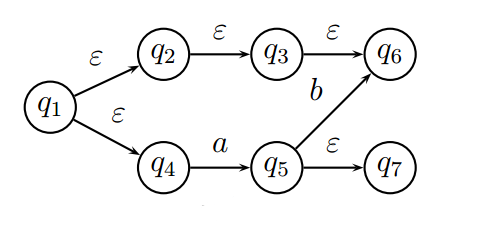
\includegraphics[scale=0.5]{18/automata.png}
\end{figure}

przykładowa odp.) $E(q_1) = \emptyset$; – tj. nie da się wyznaczyc ze względu na puste przejścia\\
\textbf{FAŁSZ}\\\\

$\varepsilon$-domknięcie stanu $q E(q)$ definiuje się:
\begin{enumerate}
\item Podstawa: Stan $q$ należy do $E(q)$
\item Krok indukcyjny: Jeżeli stan $p$ należy do $E(q)$ oraz istnieje przejście ze stanu $p$ do stanu $r$ o etykiecie $\varepsilon$, to $r$ należy do $E(q)$ - jeżeli funkcją przejścia opisywanego NAS jest $\delta$ i $p$ należy do $E(q)$, to $E(q)$ zawiera także stany z $\delta(p, \varepsilon)$.
\end{enumerate}

Dla zadanego automatu $E(q) = \{q_1, q_2, q_3, q_4, q_6\}$


%305
\answer{(K\_W15, K\_W03, K\_W04, K\_W07, K\_U15, K\_U21, K\_U22) Dany jest automat niedeterministyczny $A = \{S = \{A,B,C\}, V = \{0,1\}, \{\delta(A,1) = B, \delta(A,1) = C, \delta(B,0), \delta(C,0) = B\}, s_0 = A, Z = \{C\}\}$. Automat po determinizacji (w znaczeniu algorytmu Rabina-Scotta) będzie miał:}
{osiem stanów}
{F}
{cztery stany}
{\\
	Stworzenie deterministycznego automatu skończonego z niedeterministycznego automatu skończonego jest zawsze możliwe i otrzymany w tym procesie automat akceptuje dokładnie ten sam język, co automat wejściowy. Jeżeli niedeterministyczny automat ma $n$ stanów, wynikowy deterministyczny może mieć do $2^n$ stanów.\\
	\newline
	$S = \{A,B,C\}$ - zbiór stanów\\
	$V = \{0,1\}$ - alfabet\\
	$\delta(A,1) = B, \delta(A,1) = C, \delta(B,0), \delta(C,0) = B$ - funkcje przejścia\\
	$s_0 = A$ - stan początkowy\\
	$Z = \{C\}$ - stany końcowe (akceptujące)\\
	Powyższy automat wygląda jak na rysunku \ref{a}.\\
	\newline
	Automat skończony, deterministyczny i zupełny nazywamy deterministycznym automatem Rabina-Scotta.\\
	Automat skończony $A$ jest deterministyczny i zupełny $\Leftrightarrow$\\($\forall s\in S: \#\delta(s,\epsilon) = 0$) $\wedge$ ($\forall a \in V: \forall s \in S: \#\delta(s,a) = 1$)\\
	\newline
	Maksymalna liczba stanów w deterministycznym automacie wynosi $2^3 = 8$.\\
	Tworzymy automat z $8$ stanami, tak żeby z każdego stanu wychodziła jedna strzałka z $1$ oraz jedna z $0$ (rys. \ref{b}):\\
	$S' = \{\alpha, \beta, \gamma, \alpha\beta, \alpha\gamma, \beta\gamma, \alpha\beta\gamma, \omega\}$:\\
	$\alpha$ odpowiada stanowi $A$, $\beta$ - $B$, $\gamma$ - $C$,\\ 
	$\omega$ - jeżeli z któregoś stanu nie istnieje przejście dla $1$ lub $0$ do innego stanu, wtedy przejście jest do $\omega$,\\ 
	każdy ze stanów $\alpha\beta, \alpha\gamma, \beta\gamma, \alpha\beta\gamma$ odpowiada za wszystkie stany, które zawiera, tzn. np. dla stanu $\beta\gamma$ z $A$($\alpha$) można przejść($1$) zarówno do $B$($\beta$) jak i do $C$($\gamma$), to znaczy, że istnieje połączenie($1$) z $\alpha$ do $\beta\gamma$; ani z $B$ ani z $C$ nie ma przjeścia dla $1$, więc z $\beta\gamma$ dla $1$ jest przejście do $\omega$, natomiast $0$ jest osiągalne z $B$ do $A$ oraz z $C$ do $B$, więc z $\beta\gamma$ jest strzałka($0$) do $\alpha\beta$. I tak postepujemy dla wszystkich nowych stanów tworząc połączenia.\\
	$V' = \{0,1\}$ - nic się nie zmienia\\
	funkcje przejścia widać na rysunku \ref{b}\\
	$s_0' = \alpha$ - nowy stan początkowy\\
	$Z' = \{\gamma, \alpha\gamma, \beta\gamma, \alpha\beta\gamma\}$ - wszystkie stany, które zawierają $\gamma$($C$)\\
	\newline
	Ostatnią rzeczą jest usunięcie stanów, do których nie da się przejść ze stanu początkowego(są one bezużyteczne), czyli zaczynając od stanu $\alpha$ sprawdzamy do których stanów istnieje ścieżka. Gotowy graf przedstawia rysunek \ref{c} - $4$ stany.
	
	
	\begin{figure}[h]
%		\includegraphics[width=0.3\textwidth]{naut}
%		\includegraphics[width=0.3\textwidth]{daut1}
%		\includegraphics[width=0.3\textwidth]{daut2}
		\centering
		\subfloat[automat niedeterministyczny]{\label{a}
			\includegraphics[width=0.3\textwidth]{18/naut}}
		\quad
		\subfloat[automat po determinizacji z nieosiągalnymi stanami]{\label{b}
			\includegraphics[width=0.3\textwidth]{18/daut1}}
		\quad
		\subfloat[automat po determinizacji bez nieosiągalnych stanów]{\label{c}
			\includegraphics[width=0.3\textwidth]{18/daut2}}
		\caption{}
	\end{figure}
}

%306
\answer
{Jeżli $r$ oraz $s$ są wyrażeniami regularnymi dla języków odpowiednio $R$ oraz $S$, to $(r+s)$, $rs$ i $r^*$ są wyrażeniami regularnym reprezentującymi odpowiednio}
{ $R \cup S$, $R \times S$ i $R^+$}
{F}
{$R \cup S$, $R \times S$ i $R^*$}
{
	$(r+s) \rightarrow r | q$, oznacza sumę teoriomnogościową języków $R$ i $S$. $R \cup S = \{x | x \in R \lor x \in S\}$ \\
	$rs$, oznacza złożenie (konkatenację) języków $R$ i $S$. $R \times S = \{rs | r \in R, s \in S\}$ \\
	$r^*$, oznacza domknięcie Kleene'go języka $R$. $R^* = R^0 \cup R^1 \cup R^2 \cup ...$  
}

%307
\answer{(K\_W15, K\_W03, K\_W04, K\_W07, K\_U15, K\_U21, K\_U22) Wyrażenie regularne $(0 + 1)^*00(0 + 1)^*$ opisuje:}
{łańcuchy rozpoczynające się zerem a kończące jedynką}
{F}
{wszystkie łańcuchy skłądające się z zer i jedynek, zawierające podciąg $00$}
{\\$a + b$ - alternatywa a i b (a lub b)\\
	$^*$ - domknięcie Kleene'ego\\ 
	$ab$ - złożenie a i b (litery występują razem w tej kolejności)\\
	$a^* = \{\epsilon, a, aa, aaa, ...\}$\\
	$(a + b)^* = \{\epsilon, a, aa, b, bb, ab, ba, abb, ...\}$ - każde możliwe słowo składające się z liter a i b}

%308
\section{K\_W15, K\_W03, K\_W04, K\_W07, K\_U15, K\_U21, K\_U22}
\textbf{308. Mamy języki $L_1 = \{ a^{2^n} : n > 0\}$ oraz $L_2 = \{ a^{2n} : n > 0\}$. Które z tych języków są regularne? }\\
przykładowa odp.) $L_1$ -- tak, $L_2$ -- tak\\
\textbf{FAŁSZ}\\\\

\textbf{Język regularny} -- język formalny taki, że istnieje automat o skończonej liczbie stanów potrafiący zdecydować, czy dane słowo należy do języka.\\\\

Wykorzystując lemat o pompowaniu należy pokażać, że język jest nieregularny. Dla $L_1$:\\
\begin{enumerate}
	\item Wybieramy x,y,z takie, że : $x=\varepsilon, y=a^{2^{k}-1}, z=a$
	\item Słowo składa się wyłącznie z liter $a$ oraz $0<|v|<2^k$
	\item Dla $i=2$ słowo $xuv^2wz \notin L_1 $, bo $2^k < |xuv^2wz| < 2^{k+1}$
\end{enumerate}
Zatem $L_1$ jest językiem nieregularnym
